\documentclass[11pt,a4paper]{article}

% ----------------------------------------------------------------------------
%  A 6502 Home Computer in Reconfigurable Logic
%  Technical project paper -- Rudolf Stepan
% ----------------------------------------------------------------------------

\usepackage[T1]{fontenc}
\usepackage[utf8]{inputenc}
\usepackage{mathpazo}              % Palatino body (warm editorial tone)
\usepackage[scaled=0.90]{helvet}  % Helvetica for headings / sans
\usepackage{courier}              % monospaced for code & registers
\usepackage{microtype}
\usepackage{amsmath}              % \text in the combined-IRQ expression

\usepackage[a4paper,margin=2.4cm]{geometry}
\usepackage{graphicx}
\usepackage{xcolor}
\usepackage{booktabs}
\usepackage{array}
\usepackage{caption}
\usepackage{enumitem}
\usepackage{titlesec}
\usepackage{fancyhdr}
\usepackage{listings}
\usepackage{tikz}
\usetikzlibrary{positioning,arrows.meta,fit,backgrounds,calc}
\usepackage[hidelinks,colorlinks=true,allcolors=accent]{hyperref}

% Hardware screenshots live in the presentation folder; reference them by name.
\graphicspath{{../presentation/images/}{presentation/images/}}

% --- figure frame: thin panel border around screenshots --------------------
\setlength{\fboxsep}{0pt}\setlength{\fboxrule}{0.5pt}
\newcommand{\shot}[1]{{\color{panelline}\fbox{\includegraphics[width=\linewidth]{#1}}}}

% --- palette -----------------------------------------------------------------
\definecolor{accent}{HTML}{8A4B2D}     % warm sienna
\definecolor{accent2}{HTML}{2F5D62}    % muted teal
\definecolor{ink}{HTML}{1C1A17}
\definecolor{soft}{HTML}{6B6459}
\definecolor{panel}{HTML}{F4EFE7}      % warm paper panel
\definecolor{panelline}{HTML}{D8CFC0}
\definecolor{code}{HTML}{F7F4EE}

% --- section typography ------------------------------------------------------
\titleformat{\section}{\sffamily\large\bfseries\color{accent}}{\thesection}{0.6em}{}
\titleformat{\subsection}{\sffamily\normalsize\bfseries\color{accent2}}{\thesubsection}{0.6em}{}
\titlespacing*{\section}{0pt}{1.4em}{0.5em}
\titlespacing*{\subsection}{0pt}{1.0em}{0.35em}

\setlength{\parindent}{0pt}
\setlength{\parskip}{0.55em}
\renewcommand{\arraystretch}{1.25}

% --- header / footer ---------------------------------------------------------
\pagestyle{fancy}
\fancyhf{}
\renewcommand{\headrulewidth}{0.3pt}
\renewcommand{\footrulewidth}{0pt}
\fancyhead[L]{\sffamily\footnotesize\color{soft}6502 SBC FPGA}
\fancyhead[R]{\sffamily\footnotesize\color{soft}A 6502 Home Computer in Logic}
\fancyfoot[C]{\sffamily\footnotesize\color{soft}\thepage}

% --- listings ----------------------------------------------------------------
\lstdefinestyle{term}{
  basicstyle=\ttfamily\footnotesize\color{ink},
  backgroundcolor=\color{code},
  frame=single, framerule=0.4pt, rulecolor=\color{panelline},
  framesep=8pt, xleftmargin=4pt, xrightmargin=4pt,
  breaklines=true, columns=fullflexible, keepspaces=true,
  showstringspaces=false, aboveskip=10pt, belowskip=4pt
}

% --- a small panel command for callouts -------------------------------------
\newcommand{\reg}[1]{{\ttfamily #1}}

\captionsetup{font=small,labelfont={sf,bf,color=accent},textfont=it}

% ----------------------------------------------------------------------------
\begin{document}

% ====================  TITLE  ===============================================
\begin{titlepage}
\thispagestyle{empty}
\vspace*{1.2cm}
{\sffamily\bfseries\color{soft}\large SYNTHESIZABLE VHDL \quad\textbullet\quad T65 CORE \quad\textbullet\quad HARDWARE--VERIFIED}

\vspace{0.6cm}
\hrule height 1.5pt
\vspace{0.9cm}

{\sffamily\bfseries\Huge\color{ink} A 6502 Home Computer\\[2pt] Rebuilt in Logic}

\vspace{0.5cm}
{\sffamily\Large\color{accent} One machine, two implementations ---\\ an FPGA system and a software emulator\\ sharing a single memory map and ROM set}

\vspace{1.1cm}
\hrule height 0.6pt
\vspace{0.8cm}

{\large\bfseries Rudolf Stepan}\\[2pt]
{\color{soft}Independent hardware \& systems research}\\[2pt]
{\color{soft}ORCID: \href{https://orcid.org/0009-0004-2842-2579}{0009-0004-2842-2579}}\\[2pt]
{\color{soft}\href{https://stepan.science}{stepan.science} \quad\textbullet\quad \href{https://intracom.at/projects/6502_fpga_computer/}{intracom.at/projects/6502\_fpga\_computer}}

\vspace{1.4cm}

% ---- abstract panel ----
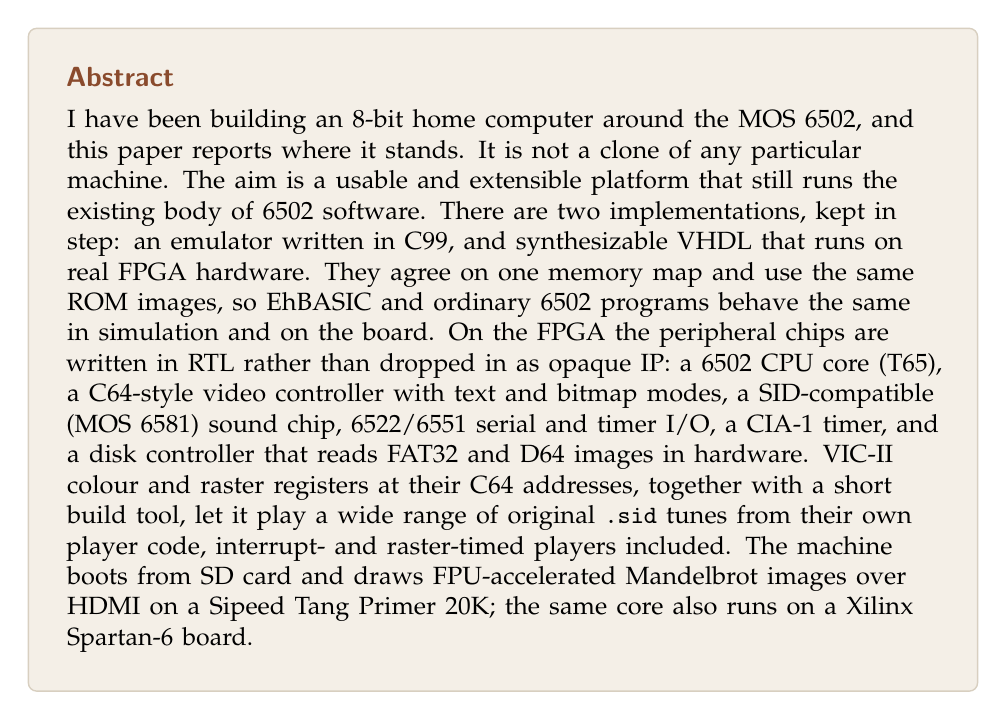
\begin{tikzpicture}
\node[fill=panel,draw=panelline,line width=0.5pt,rounded corners=3pt,
      inner sep=14pt,text width=\dimexpr\textwidth-30pt\relax] {
\begin{minipage}{\linewidth}
{\sffamily\bfseries\color{accent}Abstract}\\[4pt]
\small
I have been building an 8-bit home computer around the MOS~6502, and this
paper reports where it stands. It is not a clone of any particular
machine. The aim is a usable and extensible platform that still runs the
existing body of 6502 software. There are two implementations, kept in
step: an emulator written in C99, and synthesizable VHDL that runs on
real FPGA hardware. They agree on one memory map and use the same ROM
images, so EhBASIC and ordinary 6502 programs behave the same in
simulation and on the board. On the FPGA the peripheral chips are
written in RTL rather than dropped in as opaque IP: a 6502 CPU core
(T65), a C64-style video controller with text and bitmap modes, a
SID-compatible (MOS~6581) sound chip, 6522/6551 serial and timer I/O, a
CIA-1 timer, and a disk controller that reads FAT32 and D64 images in
hardware. VIC-II colour and raster registers at their C64 addresses,
together with a short build tool, let it play a wide range of original
\texttt{.sid} tunes from their own player code, interrupt- and
raster-timed players included. The machine boots from SD card and draws
FPU-accelerated Mandelbrot images over HDMI on a Sipeed Tang Primer~20K;
the same core also runs on a Xilinx Spartan-6 board.
\end{minipage}
};
\end{tikzpicture}

\vfill
{\color{soft}\sffamily\small Project paper \textbullet\ \today \textbullet\ Source: \href{https://github.com/rudolfstepan/6502-sbc-fpga}{github.com/rudolfstepan/6502-sbc-fpga}}
\end{titlepage}

% ====================  1. INTRODUCTION  =====================================
\section{Introduction}

The MOS~6502 is still one of the best-understood microprocessors around,
and there is a large amount of software for it that people continue to
write and maintain. New 6502 projects mostly land in one of two groups.
Some recreate a specific old computer as faithfully as possible: a
Commodore~64, an Apple~II, a BBC~Micro. Others are bare single-board
machines with a CPU, some RAM and a serial port, and not much else.

I wanted something in between. The point of this project is not to copy a
Commodore, but to design a 6502 home computer of my own that is
comfortable to use today and still compatible with classic 6502 software
where that makes sense. I define the machine once, as a memory map plus a
set of peripheral register contracts, and then build it twice: as a
software emulator and as synthesizable logic for FPGAs. Since both honour
the same addresses and registers, the same ROM images and the same
programs run on either without changes.

The rest of the paper walks through the architecture, the individual
subsystems, how each part is tested, and how far the hardware bring-up
has come.

% ====================  2. DESIGN GOALS  =====================================
\section{Design Goals}

A few decisions shaped everything that followed.

\begin{description}[leftmargin=1.4em,style=nextline,itemsep=0.3em]
  \item[\color{accent2}One machine, two implementations.]
  The emulator and the FPGA design are not two similar-looking projects.
  They are the same machine built two ways, and the memory map is the
  contract that keeps them honest.

  \item[\color{accent2}Run unmodified 6502 software.]
  EhBASIC and standalone ROM applications have to boot as-is. Whatever I
  write and debug in the emulator should run on the board, and the other
  way round.

  \item[\color{accent2}Write the chips in RTL.]
  Video, sound, timers, serial and disk are re-implemented as a
  board-independent VHDL library with the original registers at the
  original addresses, instead of being wrapped around opaque vendor IP.

  \item[\color{accent2}Be modern where it actually helps.]
  Some conveniences the 6502 era did without are worth having: HDMI
  output, an SD card for storage, a hardware multiplier. Each is reached
  through a plain memory-mapped interface the CPU can drive.

  \item[\color{accent2}Test before trusting.]
  Every block has to pass in simulation before it goes near the FPGA.
\end{description}

% ====================  3. SYSTEM OVERVIEW  ==================================
\section{System Overview}

Figure~\ref{fig:block} shows the FPGA system. A 6502-compatible CPU core
sits on a 16-bit address bus, and a combinational address decoder routes
each access to main RAM, to the banked video framebuffer, or to one of
the memory-mapped peripherals. Before any of that runs, a boot subsystem
copies the system ROM from the SD card into writable shadow RAM and only
then releases the CPU from reset.

\vspace{0.4em}
\begin{figure}[h]
\centering
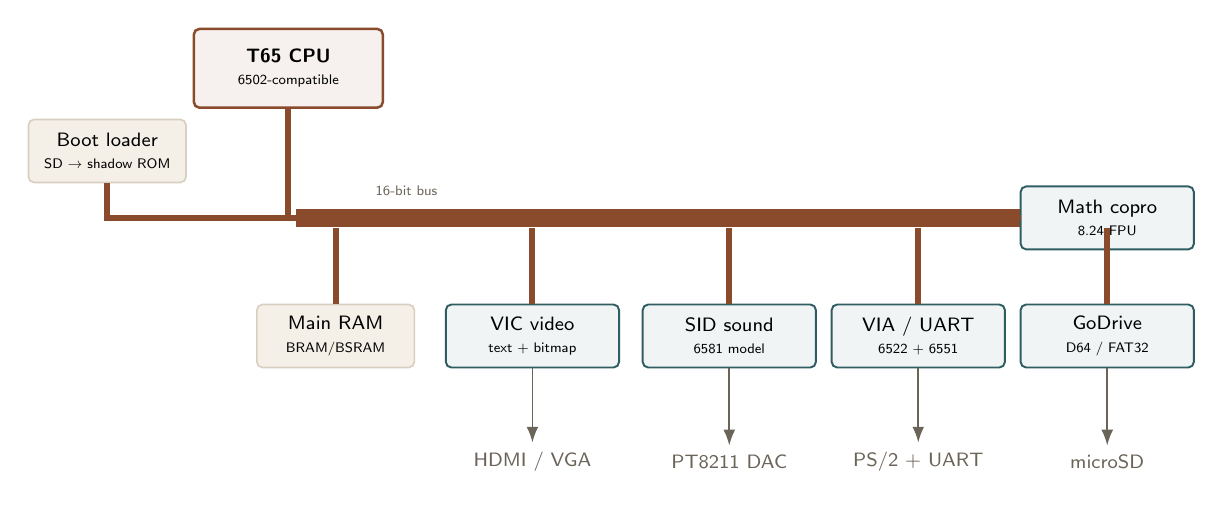
\begin{tikzpicture}[
  font=\sffamily\scriptsize,
  box/.style={draw=panelline,line width=0.6pt,fill=panel,rounded corners=2pt,
              minimum height=8mm,minimum width=20mm,align=center,inner sep=3pt},
  cpu/.style={draw=accent,line width=0.9pt,fill=accent!8,rounded corners=2pt,
              minimum height=10mm,minimum width=24mm,align=center},
  io/.style ={draw=accent2,line width=0.7pt,fill=accent2!7,rounded corners=2pt,
              minimum height=8mm,minimum width=22mm,align=center,inner sep=3pt},
  bus/.style={accent,line width=2.2pt},
  lnk/.style={-{Latex[length=2mm]},soft,line width=0.6pt}
]
% CPU
\node[cpu] (cpu) at (0,0) {\textbf{T65 CPU}\\\tiny 6502-compatible};
\node[box] (boot) at (-2.3,-1.05) {Boot loader\\\tiny SD $\to$ shadow ROM};
% the bus
\node[draw=none,fill=accent,minimum width=92mm,minimum height=2.4pt] (bus) at (4.7,-1.9) {};
\node[soft,font=\sffamily\tiny] at (1.5,-1.55) {16-bit bus};
\draw[bus] (cpu.south) |- (bus.west);
\draw[bus] (boot.south) |- (bus.west);

% peripherals along the bus
\node[box] (ram)  at (0.6,-3.4) {Main RAM\\\tiny BRAM/BSRAM};
\node[io]  (vic)  at (3.1,-3.4) {VIC video\\\tiny text + bitmap};
\node[io]  (sid)  at (5.6,-3.4) {SID sound\\\tiny 6581 model};
\node[io]  (via)  at (8.0,-3.4) {VIA / UART\\\tiny 6522 + 6551};
\node[io]  (d64)  at (10.4,-3.4){GoDrive\\\tiny D64 / FAT32};
\node[io]  (fpu)  at (10.4,-1.9){Math copro\\\tiny 8.24 FPU};

\foreach \n in {ram,vic,sid,via,d64} \draw[bus] (\n.north) -- (\n.north|-bus.south);
\draw[bus] (fpu.west) -- (fpu.west-|bus.east);

% outputs
\node[draw=none,soft] (hdmi) at (3.1,-5.0) {HDMI / VGA};
\node[draw=none,soft] (dac)  at (5.6,-5.0) {PT8211 DAC};
\node[draw=none,soft] (kbd)  at (8.0,-5.0) {PS/2 + UART};
\node[draw=none,soft] (sd)   at (10.4,-5.0){microSD};
\draw[lnk] (vic.south) -- (hdmi.north);
\draw[lnk] (sid.south) -- (dac.north);
\draw[lnk] (via.south) -- (kbd.north);
\draw[lnk] (d64.south) -- (sd.north);
\end{tikzpicture}
\caption{Block diagram of the FPGA system. The board-independent RTL
core (CPU, bus, RAM, and the memory-mapped peripheral library) is shared
across both FPGA targets; only thin board glue differs.}
\label{fig:block}
\end{figure}

The same specification also drives the reference emulator, a C99 program
with an SDL2 backend and an interactive monitor. The FPGA repository
pulls in the emulator's ROM and kernel sources directly, so the two
tracks cannot drift apart without someone noticing at build time.
Figure~\ref{fig:boot} shows the FPGA build sitting at the EhBASIC prompt.

\begin{figure}[h]
\centering
\begin{minipage}{0.62\linewidth}\shot{tang_primer_ehbasic_boot.jpg}\end{minipage}
\caption{Enhanced~BASIC booting on the HDMI output of the Tang Primer~20K.
The banner is drawn by the kernel's self-test before control passes to the
BASIC interpreter; the same ROM image runs unchanged in the emulator.}
\label{fig:boot}
\end{figure}

% ====================  4. CPU  ==============================================
\section{Processor Core}

The CPU is the open-source \textbf{T65} soft core, a 6502-compatible
processor written in VHDL. A small project-local adapter sits between the
core and the system: it narrows the core's wide internal address bus to
16 bits, exports the write-enable and write-data signals, and feeds read
data from memory and peripherals back in. A \reg{cpu\_enable} toggle lets
the processor step on every other system clock, which gives an effective
CPU rate of up to \textbf{27\,MHz} and still leaves a settled bus phase
for the synchronous FPGA memories. Interrupts work as on the real part:
the reset vector comes from \reg{\$FFFC}, and maskable interrupts vector
through \reg{\$FFFE/\$FFFF}.

That half-rate stepping is the trick that makes the rest easy. The 6502
bus expects asynchronous-style reads, but block RAM on an FPGA is
synchronous. Registering read data during the settled half of each cycle
reconciles the two and keeps the simulation timing deterministic.

% ====================  5. MEMORY MAP  =======================================
\section{Memory Map}

If anything is the heart of the project, it is the memory map: the one
contract both implementations honour. Table~\ref{tab:map} lists the
configuration currently running on the Tang Primer~20K.

\begin{table}[h]
\centering
\small
\begin{tabular}{@{}>{\ttfamily}l l l@{}}
\toprule
\textnormal{\textbf{Range}} & \textbf{Size} & \textbf{Device} \\
\midrule
\$0000--\$3FFF & 16\,KB & BRAM main RAM --- zero page, stack, EhBASIC \\
\$4000--\$5FFF & 8\,KB  & BSRAM main RAM (optional DDR3 backend) \\
\$6000--\$7FFF & 8\,KB  & Window into the banked VIC framebuffer \\
\$8000--\$87FF & 2\,KB  & VIC text \& colour RAM \\
\$8800--\$880F & 16\,B  & VIA 6522 \\
\$8810--\$8813 & 4\,B   & UART 6551 \\
\$8820--\$8823 & 4\,B   & Keyboard (PS/2 controller; USB-HID prepared) \\
\$8824         & ---    & D64 GoDrive registers \\
\$88B0--\$88BF & 16\,B  & Math coprocessor (8.24 FPU) \\
\$9000--\$900F & 16\,B  & VIC control registers \\
\$D000--\$D03F & 64\,B  & VIC-II registers (border/bg + \$D011/\$D012 raster) \\
\$A000--\$CFFF & 12\,KB & Shadow-ROM application window \\
\$D400--\$D41C & 29\,B  & SID-compatible audio registers (incl. OSC3/ENV3) \\
\$DC00--\$DC0F & 16\,B  & CIA-1 --- Timer A + interrupt control \\
\$F000--\$FFFF & 4\,KB  & Shadow-ROM kernel \& vectors \\
\bottomrule
\end{tabular}
\caption{Active Tang Primer~20K memory map. The C64-compatible VIC-II
(\$D020/\$D021, \$D011/\$D012), SID (\$D400) and CIA-1 (\$DC00) blocks sit at
their original addresses, so classic \reg{POKE}s and SID players work
unchanged. The physical shadow-ROM image is 16\,KB: offsets
\reg{\$0000--\$2FFF} map to \reg{\$A000--\$CFFF}, and \reg{\$3000--\$3FFF}
map to \reg{\$F000--\$FFFF}.}
\label{tab:map}
\end{table}

% ====================  6. VIDEO  ============================================
\section{Video Subsystem (VIC)}

The video controller re-implements a C64-style display in RTL, with its
own horizontal and vertical sync generation, character-ROM lookup, and a
16-colour Pepto-style palette.

\subsection{Display modes}

The controller supports a text mode and four bitmap modes:

\begin{itemize}[leftmargin=1.4em,itemsep=0.2em]
  \item \textbf{40$\times$25 text} --- each cell scaled to 16$\times$16
  screen pixels, with per-cell foreground/background colour from the
  colour RAM at \reg{\$8400} and an 8$\times$8 glyph from a 256-entry
  character ROM.
  \item \textbf{320$\times$240, 16 colours (4\,bpp)} --- a full-screen
  bitmap held in a dedicated on-chip framebuffer, displayed 1:1 and
  centred, with the surrounding border filled in the \reg{\$D020} colour.
  \item \textbf{320$\times$200 1-bpp} --- legacy bitmap, 2$\times$ scaled
  to 640$\times$400, 16 colours per 8$\times$8 cell.
  \item \textbf{160$\times$100 RGB332} --- 256 colours, one byte per
  pixel, 4$\times$ scaled.
  \item \textbf{180$\times$120 RGB222} --- 64 colours packed four pixels
  into three bytes, 3$\times$ scaled.
\end{itemize}

The framebuffer (\reg{fb\_ram}, 38\,400 bytes for 320$\times$240 at
4\,bpp) is reached through an 8\,KB CPU window at \reg{\$6000--\$7FFF};
in the 16-colour mode three bank bits in \reg{\$9000[7:5]} slide that
window across the buffer, while the \reg{\$9000} MODE register selects
the active display format. Figure~\ref{fig:bitmap} shows two of the
bitmap modes running on the board, and Figure~\ref{fig:text} the text
mode alongside the 1-bpp bitmap.

\begin{figure}[h]
\centering
\begin{minipage}{0.48\linewidth}\shot{tang_primer_mandelbrot_col.jpg}\end{minipage}\hfill
\begin{minipage}{0.48\linewidth}\shot{tang_primer_bitmap_mode.jpg}\end{minipage}
\caption{Bitmap graphics from the running board. \textit{Left:} an
FPU-accelerated 256-colour Mandelbrot set in the RGB332 mode.
\textit{Right:} direct-from-BASIC pixel plotting. Both are photographed
from the HDMI output, not rendered.}
\label{fig:bitmap}
\end{figure}

\subsection{Bus stealing --- the shared bus}

VIC and CPU share a single-port video memory. During each horizontal
blanking interval the VIC prefetches the next display line and holds the
CPU through the \reg{RDY} pin. The measured overhead is small ---
\textbf{4.8\,\%} in text mode, up to 9.4\,\% in the heaviest bitmap mode
--- and CPU writes to video RAM are never lost: a pending write is
buffered and committed on the first free clock.

\subsection{C64-compatible VIC-II registers}

For software compatibility the controller also exposes a VIC-II register
block at the original C64 addresses, \reg{\$D000--\$D03F}. The border
(\reg{\$D020}) and global background (\reg{\$D021}) colours respond to the
classic \reg{POKE 53280,c} / \reg{POKE 53281,c}, and the rest of the
block is a read/write register file. Two registers are \emph{live} on
read: \reg{\$D012} gives back the current raster line (its low eight
bits) and \reg{\$D011} bit~7 carries raster bit~8. That small detail
earns its place. A raster-synchronised player, or any old timing loop
that busy-waits on \reg{\$D012}, would otherwise compare against a fixed
value and never move on. With the scan counter actually running, the wait
completes. Section~\ref{sec:audio} comes back to this for SID playback.
Figure~\ref{fig:colorreg} shows the border and background colours set
from BASIC with \reg{POKE}.

\begin{figure}[h]
\centering
\begin{minipage}{0.48\linewidth}\shot{color_border_bg_demo1.jpg}\end{minipage}\hfill
\begin{minipage}{0.48\linewidth}\shot{color_border_bg_demo2.jpg}\end{minipage}
\caption{The C64-compatible colour registers driven from BASIC.
\reg{POKE 53280,c} sets the border (\reg{\$D020}) and \reg{POKE 53281,c}
the background (\reg{\$D021}); the two captures use different border
colours over the same blue background.}
\label{fig:colorreg}
\end{figure}

\subsection{Output}

On the Tang Primer~20K the controller drives a DVI-style \textbf{HDMI}
output at \textbf{720$\times$480p} (exact CEA-861 480p timing, 640-wide
content pillar-boxed) through a TMDS serializer, with a 27\,MHz pixel
clock and a 135\,MHz TMDS clock. An AVI InfoFrame is emitted alongside
the video so that USB HDMI capture devices --- which, unlike most
monitors, reject a bare DVI signal --- lock onto the format. The
Spartan-6 reference board instead produces VGA text output with a boot
status screen.

\begin{figure}[h]
\centering
\begin{minipage}{0.48\linewidth}\shot{tang_primer_petscii_test.jpg}\end{minipage}\hfill
\begin{minipage}{0.48\linewidth}\shot{tang_primer_mandelbrot_bw.jpg}\end{minipage}
\caption{\textit{Left:} PETSCII block and line graphics in the 40$\times$25
text mode. \textit{Right:} a monochrome Mandelbrot in the 320$\times$200
1-bpp bitmap mode.}
\label{fig:text}
\end{figure}

% ====================  7. AUDIO  ============================================
\section{Audio Subsystem (SID-compatible)}\label{sec:audio}

The sound chip is a fairly complete model of the \textbf{MOS~6581
(SID)}. It provides three independent voices with combined waveforms,
ADSR envelopes built on the reSID rate-counter periods, and a
two-pole state-variable multimode filter (low/band/high pass) with a
deliberately ``dark 6581'' cutoff curve. Each oscillator is built on a
24-bit phase accumulator; the register file occupies \reg{\$D400--\$D41C}
in keeping with the original layout (the read-only OSC3/ENV3 registers at
\reg{\$D41B/\$D41C} are included). Audio leaves the FPGA through a PT8211
I\textsuperscript{2}S DAC at roughly 47\,kHz.

The hardest thing I ask of it is to play \textbf{original \texttt{.sid}
files together with their 6502 player code}, directly on the hardware.
The same routines that would drive a real SID drive this RTL model
instead, and the music comes out recognisable. The rest of this section
is about how an arbitrary tune gets wrapped to run on the bare machine.

\subsection{Wrapping a tune}

The tool \reg{build\_native\_sid\_rom.py} turns a PSID/RSID file into a
standalone ROM. It does \emph{not} perform a lossy 50\,Hz register dump;
instead it embeds the tune's original 6502 payload, places it at its
native load address, calls the tune's \reg{init} routine once, and then
drives the tune's \reg{play} routine. Every frequency, pulse-width,
control, ADSR and filter write therefore reaches the hardware exactly as
the original player produces it.

Two load layouts are chosen automatically from the tune's load address.
A tune that loads into linear RAM (\reg{\$0200--\$5FFF}) is embedded in a
wrapper at \reg{\$A000} that copies the payload down to its load address.
A tune that loads at \reg{\$A000--\$CFFF} is handled by a
\emph{RAM-under-BASIC} ``page'' layout: the EhBASIC shadow ROM is made
CPU-writable in that window so the tune sits directly at its native
address with no copy, and a small player lives at \reg{\$F000}.

The \reg{play} address selects one of two drive paths:

\begin{description}[leftmargin=1.2em,style=nextline,itemsep=0.25em]
  \item[\color{accent2}Polled (\reg{play}\,$\neq$\,0).]
  \reg{init} runs once, then \reg{play} is called every $\approx$20\,ms
  off the millisecond counter at \reg{\$883A}. This needs no interrupt
  and never depends on the CIA or VIC. A free-running CIA Timer~A is also
  started so tunes that \emph{read} \reg{\$DC04} see a live timer.
  \item[\color{accent2}Interrupt-driven (\reg{play}\,=\,0).]
  The tune installs its own CIA timer and \reg{\$0314} handler in
  \reg{init}; the wrapper supplies only a default vector and a
  \reg{\$FFFE\,$\to$\,JMP (\$0314)} bridge. This path uses the CIA-1
  Timer~A described in Section~\ref{sec:io}.
\end{description}

After \reg{init} the wrapper always executes \reg{SEI}. Some RSID
\reg{init} routines end with \reg{CLI}, expecting to run under their own
interrupt; without re-masking, a stray IRQ would vector through the ROM
\reg{\$FFFE} bridge into an uninitialised \reg{\$0314} and crash. For an
ordinary tune whose \reg{init} does not touch the interrupt flag, the
\reg{SEI} is a harmless no-op.

\subsection{Case study: a raster-timed player}

A handful of RSID tunes do not fit either drive path cleanly. They
declare \reg{play\,=\,\$0000}, yet they are not silent: their real
per-frame update is buried inside a \textbf{VIC raster-interrupt} handler.
The tune \textit{Arkanoid} is a good example. Disassembling its
\reg{init} (\reg{\$4000}) shows it switch the C64
memory banks via \reg{\$01}, write its own handler vector straight into
\reg{\$FFFE/\$FFFF}, enable a raster interrupt through \reg{\$D01A}, and
\reg{CLI}. Its handler acknowledges the VIC, programs the next raster
compare line, and calls the actual SID update at \reg{\$4141}.

None of that survives on the bare machine: the FPGA generates no VIC
raster interrupts, \reg{\$FFFE/\$FFFF} is read-only kernel ROM, and there
is no \reg{\$01} banking. The fix sidesteps the interrupt entirely. A
small per-tune \emph{override table} in the build tool points \reg{play}
at the inner update routine (\reg{\$4141}) discovered by disassembly, so
the \emph{polled} path drives it directly at 50\,Hz. Because that tune's
\reg{init} performs a \reg{CLI}, the \reg{SEI}-after-\reg{init} guard
above is what keeps it from crashing. With both pieces in place the tune
plays from its own unmodified player code, with no interrupt at all.

\subsection{Building a collection}

A companion tool, \reg{build\_all\_sid\_roms.py}, wraps every suitable
tune in a folder, emitting a ROM and an upload script for each. By
default it first runs each tune through a bare-metal 6502 SID emulator and
\emph{skips} tunes that never set the master volume or gate a voice ---
they would be silent on this hardware. Hand-made demonstration ROMs are
protected by a \texttt{CURATED} list and are never overwritten by the
bulk build.

\begin{lstlisting}[style=term]
# wrap one tune
python tools/build_native_sid_rom.py path/to/tune.sid sw/<name>.s

# or wrap a whole collection at once (skips silent tunes,
# keeps curated ROMs, links page-mode tunes automatically)
python tools/build_all_sid_roms.py
\end{lstlisting}

% ====================  8. IO  ===============================================
\section{Timers, Serial, and Input}\label{sec:io}

Three classic-style chips round out the I/O. The \textbf{VIA 6522}
(\reg{\$8800}) provides timers, general-purpose I/O ports, and interrupt
flags; its Timer~1 supplies the kernel's periodic tick, and Port~B bit~0
drives the board LED after boot. The \textbf{UART 6551} (\reg{\$8810})
implements full transmit and receive logic with status registers and a
receive interrupt; on the host side it appears as a CH340 serial port at
115200~8N1.

A \textbf{CIA-1} (\reg{\$DC00--\$DC0F}) adds a MOS-6526 subset for C64
compatibility: a Timer~A down-counter with latch (\reg{\$DC04/\$DC05}), a
control register (\reg{\$DC0E}) for start, one-shot and force-load, and an
interrupt control register (\reg{\$DC0D}) whose mask is set or cleared by
the high bit of the written value and whose status is cleared on read.
This is what lets interrupt-driven SID players raise their player from a
Timer-A interrupt exactly as on a real C64.

Keyboard input takes a small shortcut. A \textbf{PS/2 keyboard} on a PMOD
connector has its keystrokes fed straight into the UART receive path, so
EhBASIC and the rest of the firmware read typed characters as ordinary
serial input and need no keyboard driver of their own. A generic switches
the layout between \textbf{German and US}: Y/Z swap, the German shifted
number row, AltGr for \reg{@ \{ [ ] \} \textbackslash\ \textasciitilde\ |},
the 102nd \reg{<>|} key, and umlauts emitted as Latin-1 code points and
drawn from a 256-glyph character ROM. I tried a USB-HID bit-bang host
first, but it never enumerated reliably, so PS/2 won; the USB-HID register
window is \emph{prepared} in the map but is not the active input.

All maskable interrupt sources are OR-combined into the single 6502
\reg{IRQ} line, $\overline{\text{\reg{irq}}} = \lnot(\text{via} \lor
\text{uart} \lor \text{kbd} \lor \text{disk} \lor \text{cia-1})$, and the
CPU vectors through \reg{\$FFFE/\$FFFF} as usual.

% ====================  9. STORAGE  ==========================================
\section{Mass Storage: D64 GoDrive}

Programs are loaded through a virtual disk drive I call \textbf{GoDrive}.
A second SD card, formatted FAT32, holds \texttt{.d64} disk images. What
is unusual is where the parsing happens. The FPGA reads both the FAT32
file system \emph{and} the D64 image format \textbf{in logic}, and hands
the 6502 nothing but plain 256-byte sectors at \reg{\$8824}. No
file-system code runs on the CPU at all.

To whoever is typing, it behaves like an old disk drive. The familiar
BASIC commands work directly:

\begin{lstlisting}[style=term]
EhBASIC ready.
LOAD "$"
 0  "TESTDISK     " 1A 2A
   4  "HELLO"          PRG
   8  "MANDELBROT"     PRG
  12  "SOUNDDEMO"      PRG
READY.
LOAD "HELLO"
LOADING... $0801-$08C9
CALL 2049
HELLO FROM A REAL 6502!
READY.
\end{lstlisting}

The drive autodetects MBR-partitioned cards and ``superfloppy''
layouts, offers an interactive arrow-key selection menu
(\reg{LOAD~"!"}), and has been verified on a real 32\,GB
Windows-formatted SD card. The D64 container is borrowed purely for
convenience: the programs it holds are this system's own code and are
\emph{not} C64-compatible.

% ====================  10. COPRO  ===========================================
\section{Math Coprocessor}

Arithmetic-heavy BASIC programs get help from a memory-mapped
\textbf{FPU} at \reg{\$88B0}, which does signed 32$\times$32 fixed-point
multiplication in \textbf{8.24 format}. That is what makes the Mandelbrot
renderings bearable from BASIC: the inner-loop multiplies go to hardware
rather than being built up from 8-bit 6502 multiply routines.
Figure~\ref{fig:asm} shows one such render driven from hand-written
assembly.

\begin{figure}[h]
\centering
\begin{minipage}{0.6\linewidth}\shot{tang_primer_mandelbrot_asm_fixed.jpg}\end{minipage}
\caption{A Mandelbrot set computed in hand-written 6502 assembly using
fixed-point arithmetic, with the inner multiplications handed to the
memory-mapped coprocessor.}
\label{fig:asm}
\end{figure}

% ====================  11. BOOT  ============================================
\section{Boot and Clocking}

A single 27\,MHz oscillator feeds a 270\,MHz PLL, and the TMDS, system
and pixel clocks are divided down from there. At power-on the board works
through a short sequence before the CPU ever runs:

\vspace{0.3em}
\begin{tikzpicture}[font=\sffamily\scriptsize,node distance=3.5mm,
  bootstep/.style={draw=panelline,fill=panel,rounded corners=2pt,line width=0.5pt,
               minimum height=11mm,text width=23mm,align=center,inner sep=3pt},
  ar/.style={-{Latex[length=2mm]},accent,line width=0.8pt}]
\node[bootstep] (a) {\textbf{1. microSD}\\\tiny SPI mode reads boot image};
\node[bootstep,right=of a] (b) {\textbf{2. sd\_rom\_loader}\\\tiny validates sector 0, streams 1\dots32};
\node[bootstep,right=of b] (c) {\textbf{3. shadow ROM}\\\tiny 16\,KB window loaded};
\node[bootstep,right=of c] (d) {\textbf{4. self-test}\\\tiny RAM\,$\cdot$\,VRAM\,$\cdot$\,VIA\,$\cdot$\,UART};
\node[bootstep,right=of d] (e) {\textbf{5. T65 release}\\\tiny reset vector @ \$FFFC};
\draw[ar] (a)--(b); \draw[ar] (b)--(c); \draw[ar] (c)--(d); \draw[ar] (d)--(e);
\end{tikzpicture}
\vspace{0.3em}

The boot image survives a reset. While I am working on firmware, a
built-in UART monitor can also write straight into the shadow-ROM RAM
over the serial link, so a fresh ROM can be uploaded and run without
touching the SD card. That copy is volatile: the next reset brings back
the SD image.

% ====================  12. VERIFICATION  ====================================
\section{Verification}

Every block runs on its own in simulation under \textbf{GHDL} before it
goes near the FPGA; Table~\ref{tab:tests} summarises what the testbenches
currently cover. The emulator pulls its weight here too. It runs the
\textbf{Klaus Dormann} 6502 functional test suite as part of its normal
build, so the instruction semantics both tracks rely on are checked
against an outside reference rather than against my own assumptions.

\begin{table}[h]
\centering
\small
\begin{tabular}{@{}l p{0.66\linewidth}@{}}
\toprule
\textbf{Area} & \textbf{Coverage} \\
\midrule
Bus \& reset & Address decoding of all device windows; reset-vector fetch; ROM-scripted bus cycles \\
VIA 6522     & Port masking; IER/IFR; Timer-1 IRQ assertion and clearing \\
UART 6551    & Status, TX, RX, overrun, programmed reset, RX IRQ \\
T65 CPU      & Boot from real ROM; UART/VIA access; IRQ handler; kernel smoke test \\
D64 / FAT32  & Real-geometry images read lazily; start LBAs verified \\
SID \& FPU   & SID audio/filter bounded and non-silent; 8.24 multiply checked against a reference \\
\bottomrule
\end{tabular}
\caption{Incremental GHDL testbench coverage, from address decoding up to
the FAT32 reader.}
\label{tab:tests}
\end{table}

% ====================  13. PORTABILITY  =====================================
\section{Portability: One Core, Two Boards}

The board-independent RTL core runs on two FPGA targets with only thin
board-specific glue, summarised in Table~\ref{tab:boards}.

\begin{table}[h]
\centering
\small
\begin{tabular}{@{}l l l@{}}
\toprule
& \textbf{Tang Primer 20K} & \textbf{PIX16 board} \\
& \textit{active bring-up} & \textit{reference} \\
\midrule
FPGA      & Gowin GW2A-18 & Xilinx Spartan-6 xc6slx16 \\
Video     & HDMI/DVI via TMDS & VGA text + boot status \\
Main RAM  & BSRAM (DDR3 optional) & SDRAM with self-test \\
Boot      & On-board microSD (SPI) & SD boot of 16\,KB shadow ROM \\
Sound     & Native SID via PT8211 DAC & --- \\
Input     & PS/2 over PMOD, CH340 UART & UART monitor \\
Toolchain & Gowin project & ISE project (versioned) \\
\bottomrule
\end{tabular}
\caption{The two FPGA platforms. The Tang Primer~20K is the active
hardware bring-up target; the Spartan-6 PIX16 serves as a reproducible
reference with a live ROM-upload monitor.}
\label{tab:boards}
\end{table}

% ====================  14. EMULATOR  ========================================
\section{The Reference Emulator}

The FPGA design grew out of a companion emulator, a C99 program that came
first. It runs the MOS~6502 with all 151 official opcodes, models the same
memory-mapped VIA, UART, VIC and sound devices, draws through SDL2, and
carries an interactive monitor: registers, memory dumps, disassembly,
single-stepping, breakpoints. It ships with ready-to-run setups for
MS~BASIC and a standalone chess ROM, under the MIT licence. The FPGA build
includes the emulator's ROM and kernel sources as a submodule, which is
the mechanism that keeps both sides on the same firmware.

% ====================  15. RESULTS  =========================================
\section{Results and Current Status}

The machine runs on real hardware. On the Tang Primer~20K it boots
EhBASIC to an HDMI display, takes input from a PS/2 keyboard, loads
programs from SD through GoDrive, plays original \texttt{.sid} music
through the DAC, and draws 256-colour FPU-accelerated Mandelbrot sets,
all from the same ROM images the emulator uses. Along the way the
individual milestones have each been checked: the HDMI boot screen, the
CH340 serial port, the UART monitor that can hold the CPU and hot-upload
a ROM, the PS/2 keyboard injection, and the diagnostic that reports
correctly when no SD card is present. Figure~\ref{fig:selftest} shows that
self-test on the HDMI output.

\begin{figure}[h]
\centering
\begin{minipage}{0.6\linewidth}\shot{tang_primer_debug_screen.jpg}\end{minipage}
\caption{The power-on self-test on the HDMI output, reporting RAM, video
RAM, VIA and UART results before control is handed to the application
ROM.}
\label{fig:selftest}
\end{figure}

% ====================  16. FUTURE  ==========================================
\section{Future Work}

The roadmap continues to deepen the peripheral set rather than chase a
specific historical machine. The VIC-II compatibility layer already
provides border/background colour and live raster read-back; the natural
next step is a true \textbf{raster-compare interrupt} (with writable RAM
under the kernel vectors), which would let raster-timed players run from
their own interrupt instead of the polled work-around of
Section~\ref{sec:audio}. Further directions include VIC sprites and a
blitter, a fuller CIA implementation (Timer~B, TOD), DDR3 as the default
main-memory backend, and continued hardening of the clock-domain and
constraint work across both boards. A known open item is a T65
indirect-addressing integration case (\reg{STA (zp),Y} into video RAM),
currently quarantined as an experimental testbench outside the default
suite.

% ====================  17. CONCLUSION  ======================================
\section{Conclusion}

Treating the memory map as a contract and building to it twice keeps the
emulator and the FPGA computer in step without forcing either to give up
what it is good at. What comes out is a 6502 home computer that is modern
where modernity earns its place, with HDMI, SD storage and a hardware
multiplier, yet stays close enough to the old machines that decades-old
software, player routines and tooling still feel at home on it. I am glad
to hear feedback and ideas from anyone working with the 6502.

% ====================  RESOURCES  ===========================================
\section*{Project Resources}
\addcontentsline{toc}{section}{Project Resources}
\begin{itemize}[leftmargin=1.4em,itemsep=0.15em]
  \item Project page: \href{https://intracom.at/projects/6502_fpga_computer/}{intracom.at/projects/6502\_fpga\_computer}
  \item FPGA (RTL/sim/boards): \href{https://github.com/rudolfstepan/6502-sbc-fpga}{github.com/rudolfstepan/6502-sbc-fpga}
  \item Software emulator: \href{https://github.com/rudolfstepan/6502-sbc-emulator}{github.com/rudolfstepan/6502-sbc-emulator}
  \item Author: Rudolf Stepan --- ORCID \href{https://orcid.org/0009-0004-2842-2579}{0009-0004-2842-2579} \textbullet\ \href{https://stepan.science}{stepan.science}
\end{itemize}

% ====================  REFERENCES  ==========================================
\section*{References}
\addcontentsline{toc}{section}{References}
\small
\begin{enumerate}[label={[\arabic*]},leftmargin=2.2em,itemsep=0.2em]
  \item R.~Stepan, ``6502 SBC FPGA --- Synthesizable VHDL 6502 computer,'' project page and source repository. \href{https://github.com/rudolfstepan/6502-sbc-fpga}{github.com/rudolfstepan/6502-sbc-fpga}
  \item R.~Stepan, ``6502 SBC Emulator --- MOS~6502 SBC emulator in C99,'' source repository. \href{https://github.com/rudolfstepan/6502-sbc-emulator}{github.com/rudolfstepan/6502-sbc-emulator}
  \item D.~Wallner, ``T65 --- 6502-compatible CPU core in VHDL,'' OpenCores.
  \item L.~Davison, ``EhBASIC --- Enhanced 6502 BASIC.''
  \item K.~Dormann, ``6502/65C02 functional tests.''
  \item MOS Technology, \textit{MCS6500 Microcomputer Family Programming Manual} (6502 CPU).
  \item MOS Technology, \textit{6581 SID (Sound Interface Device) datasheet}.
  \item MOS Technology, \textit{6522 Versatile Interface Adapter (VIA) datasheet}.
  \item MOS Technology, \textit{6551 Asynchronous Communication Interface Adapter (ACIA) datasheet}.
  \item Sipeed, \textit{Tang Primer 20K (Gowin GW2A-18) documentation}.
  \item T.~Gleixner et al., ``GHDL --- open-source VHDL simulator.''
\end{enumerate}

\end{document}
